\documentclass{beamer}
\usepackage{tikz}
\usetikzlibrary{matrix,shapes,snakes}
\usepackage[absolute,overlay]{textpos}
\newcommand\circled[3]{\node(#1)[text width=.45cm,circle,draw,right of=#2,inner sep=0pt]{\tiny #3};}

\title{TP1}
\author{gar}
\date{}

\begin{document}

\maketitle

\begin{frame}[fragile]
\frametitle{Find Optimal Distribution}
\begin{itemize}
\item Find an optimal distribution such that the transportation cost is minimum
\end{itemize}

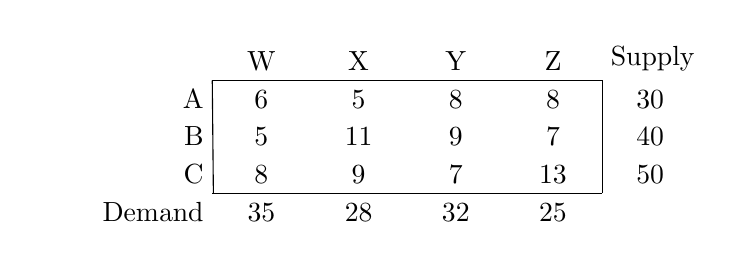
\begin{tikzpicture}
    \matrix(dict)[matrix of nodes,%below=of game,
        nodes={align=center,text width=1cm},
        row 1/.style={anchor=south},
        column 1/.style={nodes={text width=2cm,align=right}}
    ]{
         &   W  &   X  &   Y  &   Z  &  Supply  \\
 A       &   6  &   5  &   8  &   8  &      30  \\
 B       &   5  &  11  &   9  &   7  &      40  \\
 C       &   8  &   9  &   7  &  13  &      50  \\
 Demand  &  35  &  28  &  32  &  25  &          \\
    };
    \draw(dict-1-2.south west)--(dict-1-5.south east);
    \draw(dict-1-2.south west)--(dict-4-1.south east);
    \draw(dict-4-2.south west)--(dict-4-5.south east);
    \draw(dict-4-5.south east)--(dict-1-5.south east);
\end{tikzpicture}
\end{frame}

\begin{frame}[fragile]
\frametitle{Find an Initial Basic Feasible Solution}
  \begin{itemize}
  \item Find an initial BFS using any of the methods studied
  \item For this problem, the IBFS is obtained using the North West Corner Rule
  \end{itemize}

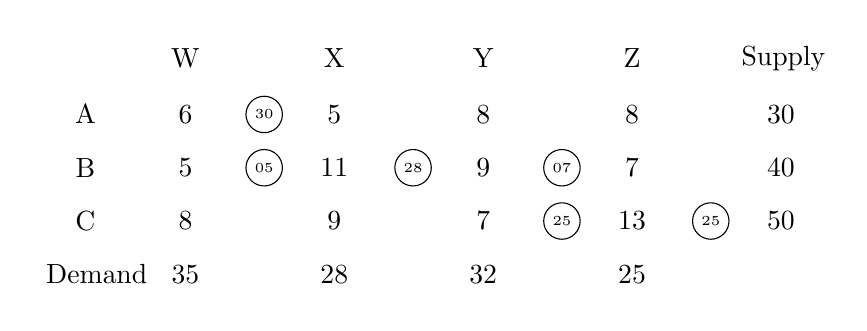
\begin{tikzpicture}
    \matrix(dd)[nodes={draw=none},align=center,text width=1cm,
        row sep=0.2cm,column sep=1pt] {
                  & \node[]{W};                            & \node[]{X};                             & \node[]{Y};                             & \node[]{Z};                             & \node[]{Supply}; \\
 \node[]{A};      & \node(d11)[]{6}; \circled{a1}{d11}{30} & \node[]{5};                             & \node[]{8};                             & \node[]{8};                             & \node[]{30};     \\
 \node[]{B};      & \node(d21)[]{5}; \circled{a2}{d21}{05} & \node(d22)[]{11}; \circled{a3}{d22}{28} & \node(d23)[]{9};  \circled{a4}{d23}{07} & \node[]{7};                             & \node[]{40};     \\
 \node[]{C};      & \node[]{8};                            & \node[]{9};                             & \node(d33)[]{7}; \circled{a5}{d33}{25}  & \node(d34)[]{13}; \circled{a6}{d34}{25} & \node[]{50};     \\
 \node[]{Demand}; & \node[]{35};                           & \node[]{28};                            & \node[]{32};                            & \node[]{25};                            &                  \\
    };
\end{tikzpicture}

\begin{itemize}
\item Now, we have the allocations, for which we are required to check for optimality
\end{itemize}
\end{frame}

\begin{frame}[fragile]
\frametitle{Iteration 0}
\begin{textblock*}{11cm}(1cm,1cm) % {block width} (coords)
  \begin{itemize}
  \only<1>{\item Make a new column $u_i$ and a new row $v_j$}
  \only<1>{\item Count the number of allocations in every row. Row A has 1, Row B has 3 and Row C has 2 allocations}
  \only<1>{\item The row which has the highest number of allocations is assigned $u_i=0$}
  \only<2->{\item For the basic variable $x_{ij}$, we must have the cost $c_{ij}=u_i+v_j$}
  \only<2>{\item Hence, from Row B costs, $c_{21} = u_2+v_1\implies 5 = 0 + v_1 \implies v_1 = 5$}
  \only<3>{\item Similarly, $c_{22} = u_2+v_2\implies 11 = 0 + v_2 \implies v_2 = 11$}
  \only<4>{\item $v_3 = 9$}
  \only<5>{\item $c_{11} = u_1+v_1\implies 6 = u_1 + 5 \implies u_1 = 1$}
  \only<6>{\item $c_{33} = u_3+v_3\implies 7 = u_3 + 9 \implies u_3 = -2$}
  \only<7>{\item $c_{34} = u_3+v_4\implies 13 = -2 + v_4 \implies v_4 = 15$}
  \end{itemize} 
\end{textblock*}  
\begin{textblock*}{5cm}(0cm,4.5cm) % {block width} (coords)
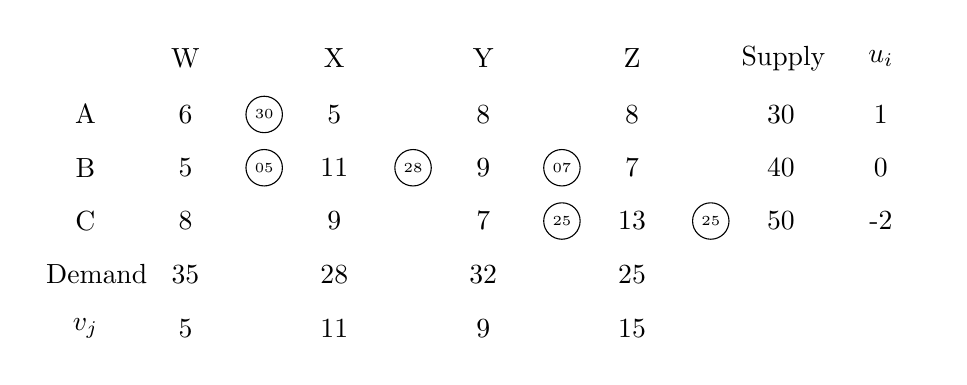
\begin{tikzpicture}
    \matrix(dd)[nodes={draw=none},align=center,text width=1cm,
        row sep=0.2cm,column sep=1pt] {
                  & \node[]{W};                            & \node[]{X};                             & \node[]{Y};                             & \node[]{Z};                             & \node[]{Supply}; & \node[]{$u_i$};            \\
 \node[]{A};      & \node(d11)[]{6}; \circled{a1}{d11}{30} & \node[]{5};                             & \node[]{8};                             & \node[]{8};                             & \node[]{30};     & \visible<5->{\node[]{1};}  \\
 \node[]{B};      & \node(d21)[]{5}; \circled{a2}{d21}{05} & \node(d22)[]{11}; \circled{a3}{d22}{28} & \node(d23)[]{9};  \circled{a4}{d23}{07} & \node[]{7};                             & \node[]{40};     & \visible<1->{\node[]{0};}  \\
 \node[]{C};      & \node[]{8};                            & \node[]{9};                             & \node(d33)[]{7}; \circled{a5}{d33}{25}  & \node(d34)[]{13}; \circled{a6}{d34}{25} & \node[]{50};     & \visible<6->{\node[]{-2};} \\
 \node[]{Demand}; & \node[]{35};                           & \node[]{28};                            & \node[]{32};                            & \node[]{25};                            &                  &                            \\
 \node[]{$v_j$};  & \visible<2->{\node[]{5};}              & \visible<3->{\node[]{11};}              & \visible<4->{\node[]{9};}               & \visible<7->{\node[]{15};}              &                  &                            \\
    };
\end{tikzpicture}
\end{textblock*}
\end{frame}

\begin{frame}
\frametitle{Iteration 0}
    \begin{itemize}
  \item After filling $u_i$ and $v_j$, compute the value $c_{ij}-u_i-v_j$ for all the nonbasic variables
  \item The obtained solution is optimal only if all the computed values are non-negative
  \item For the problem, there are several negative values, so, proceed with an iteration
  \item Determine the least value (break ties arbitrarily), and put a $\fbox{+}$ sign above the value
  \item It indicates that it is going to be allocated some value after adjusting with the adjacent allocations
  \item The chain reaction that occurs is indicated by drawing a loop, where the corners must be the allocated cells
  \item Assign alternating $+$ and $-$ signs to the corners of the loop
  \item The cells having a $+$ are called the \textit{recipient cells} and those having $-$ are called \textit{donor cells}
  \end{itemize}
\end{frame}

\begin{frame}[fragile]
\frametitle{Iteration 0}
\begin{textblock*}{11cm}(1cm,1cm) % {block width} (coords)
  \begin{itemize}
  \only<1>{\item Compute the value $c_{ij}-u_i-v_j$ for all the nonbasic variables}
  \only<1>{\item Determine the least value (break ties arbitrarily), and put a $\fbox{+}$ sign above the value}
  \only<2>{\item Starting from $\fbox{+}$, check all the 4 possible directions for an available allocation}
  \only<2>{\item Then, draw an edge to any one of it. Here, an edge is from $x_{24}$ to $x_{34}$}
  \only<3->{\item Draw another edge from $x_{34}$ to $x_{33}$}
  \only<3->{\item and continue till one loop is drawn}
  \end{itemize}
\end{textblock*}  
\begin{textblock*}{5cm}(0cm,4.5cm) % {block width} (coords)  
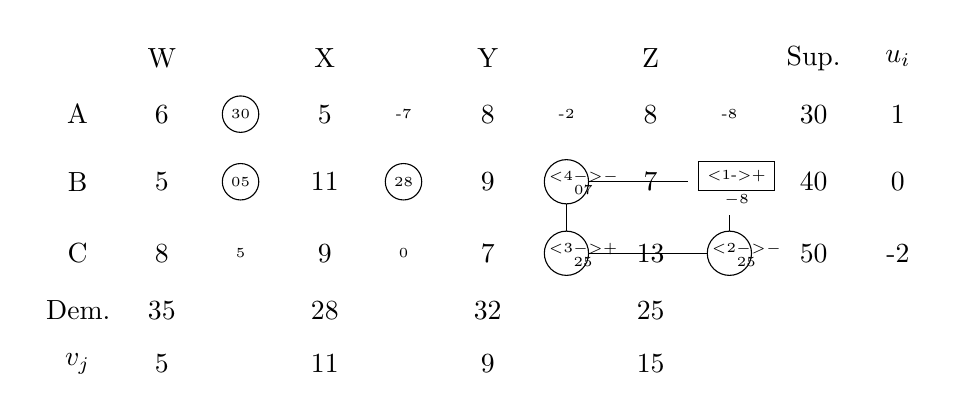
\begin{tikzpicture}
    \matrix(dd)[nodes={draw=none},align=center,text width=.8cm,
        row sep=0.2cm,column sep=1pt] {
                 & \node[]{W};                                    & \node[]{X};                                     & \node[]{Y};                                                           & \node[]{Z};                                                                              & \node[]{Sup.}; & \node[]{$u_i$}; \\
 \node[]{A};     & \node(d11)[]{6}; \circled{a1}{d11}{30}         & \node(d12)[]{5}; \node[right of=d12]{\tiny -7}; & \node(d13)[]{8}; \node[right of= d13]{\tiny -2};                      & \node(d14)[]{8}; \node[right of=d14]{\tiny -8};                                          & \node[]{30};   & {\node[]{1};}   \\
 \node[]{B};     & \node(d21)[]{5}; \circled{a2}{d21}{05}         & \node(d22)[]{11}; \circled{a3}{d22}{28}         & \node(d23)[]{9};  \circled{a4}{d23}{$\stackrel{\visible<4->{-}}{07}$} & \node(d24)[]{7}; \node(a7)[right of=d24]{\tiny $\stackrel{\fbox{\visible<1->{+}}}{-8}$}; & \node[]{40};   & {\node[]{0};}   \\
 \node[]{C};     & \node(d31)[]{8}; \node[right of=d31]{\tiny 5}; & \node(d32)[]{9}; \node[right of=d32]{\tiny 0};  & \node(d33)[]{7}; \circled{a5}{d33}{$\stackrel{\visible<3->{+}}{25}$}  & \node(d34)[]{13}; \circled{a6}{d34}{$\stackrel{\visible<2->{-}}{25}$}                    & \node[]{50};   & {\node[]{-2};}  \\
 \node[]{Dem.};  & \node[]{35};                                   & \node[]{28};                                    & \node[]{32};                                                          & \node[]{25};                                                                             &                &                 \\
 \node[]{$v_j$}; & {\node[]{5};}                                  & {\node[]{11};}                                  & {\node[]{9};}                                                         & {\node[]{15};}                                                                           &                &                 \\
    };
   \visible<2->{\draw[-](a7)--(a6);}
   \visible<3->{\draw[-](a6)--(a5);}
   \visible<4->{\draw[-](a5)--(a4);}
   \visible<5->{\draw[-](a4)--(a7);}
\end{tikzpicture}
\end{textblock*}
\end{frame}
%~ 
\begin{frame}[fragile]
\frametitle{Iteration 0}
\begin{textblock*}{11cm}(1cm,1cm) % {block width} (coords)
  \begin{itemize}
  \only<1->{\item Among the donor cells, determine the minimum value of the allocations}
  \only<1->{\item Subtract that value from all the donor cells and add that value to all the recipient cells}
  \only<2>{\item The recipient cell that had $\fbox{+}$ symbol is called the entering basic variable}
  \only<3>{\item The donor cell which loses all its allocation is called the leaving basic variable}
  \only<4>{\item If there are multiple leaving basic variables, choose one arbitrarily and assign 0 allocation to the remaining cells}
  \end{itemize}
\end{textblock*}
\begin{textblock*}{5cm}(0cm,4.5cm) % {block width} (coords)  
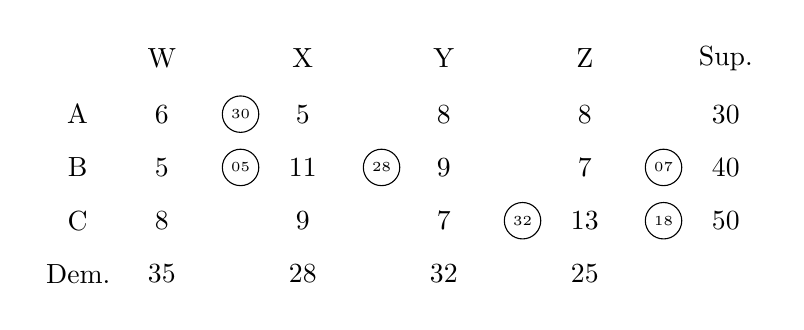
\begin{tikzpicture}
    \matrix(dd)[nodes={draw=none},align=center,text width=.8cm,
        row sep=0.2cm,column sep=1pt] {
                & \node[]{W};                            & \node[]{X};                             & \node[]{Y};                            & \node[]{Z};                             & \node[]{Sup.}; \\
 \node[]{A};    & \node(d11)[]{6}; \circled{a1}{d11}{30} & \node[]{5};                             & \node[]{8};                            & \node[]{8};                             & \node[]{30};   \\
 \node[]{B};    & \node(d21)[]{5}; \circled{a2}{d21}{05} & \node(d22)[]{11}; \circled{a3}{d22}{28} & \node(d23)[]{9};                       & \node[]{7}; \circled{a4}{d23}{07}       & \node[]{40};   \\
 \node[]{C};    & \node[]{8};                            & \node[]{9};                             & \node(d33)[]{7}; \circled{a5}{d33}{32} & \node(d34)[]{13}; \circled{a6}{d34}{18} & \node[]{50};   \\
 \node[]{Dem.}; & \node[]{35};                           & \node[]{28};                            & \node[]{32};                           & \node[]{25};                            &                \\
    };
\end{tikzpicture}
\end{textblock*}
\end{frame}

\begin{frame}[fragile]
\frametitle{Iteration 1}
  \begin{itemize}
  \item Fill in $u_i$ and $v_j$ again and check for optimality
  \end{itemize}
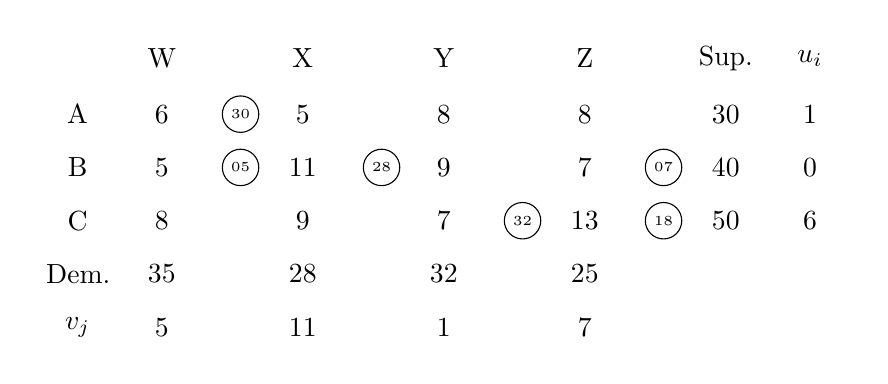
\begin{tikzpicture}
    \matrix(dd)[nodes={draw=none},align=center,text width=.8cm,
        row sep=0.2cm,column sep=1pt] {
                 & \node[]{W};                            & \node[]{X};                             & \node[]{Y};                            & \node[]{Z};                             & \node[]{Sup.}; & \node[]{$u_i$};           \\
 \node[]{A};     & \node(d11)[]{6}; \circled{a1}{d11}{30} & \node[]{5};                             & \node[]{8};                            & \node[]{8};                             & \node[]{30};   & \visible<5->{\node[]{1};} \\
 \node[]{B};     & \node(d21)[]{5}; \circled{a2}{d21}{05} & \node(d22)[]{11}; \circled{a3}{d22}{28} & \node(d23)[]{9};                       & \node[]{7}; \circled{a4}{d23}{07}       & \node[]{40};   & \visible<1->{\node[]{0};} \\
 \node[]{C};     & \node[]{8};                            & \node[]{9};                             & \node(d33)[]{7}; \circled{a5}{d33}{32} & \node(d34)[]{13}; \circled{a6}{d34}{18} & \node[]{50};   & \visible<6->{\node[]{6};} \\
 \node[]{Dem.};  & \node[]{35};                           & \node[]{28};                            & \node[]{32};                           & \node[]{25};                            &                &                           \\
 \node[]{$v_j$}; & \visible<2->{\node[]{5};}              & \visible<3->{\node[]{11};}              & \visible<7->{\node[]{1};}              & \visible<4->{\node[]{7};}               &                &                           \\
    };
\end{tikzpicture}
\end{frame}

\begin{frame}[fragile]
\frametitle{Iteration 1}
  \begin{itemize}
  \item Since it's not optimal, again draw a loop and redistribute the allocations
  \end{itemize}
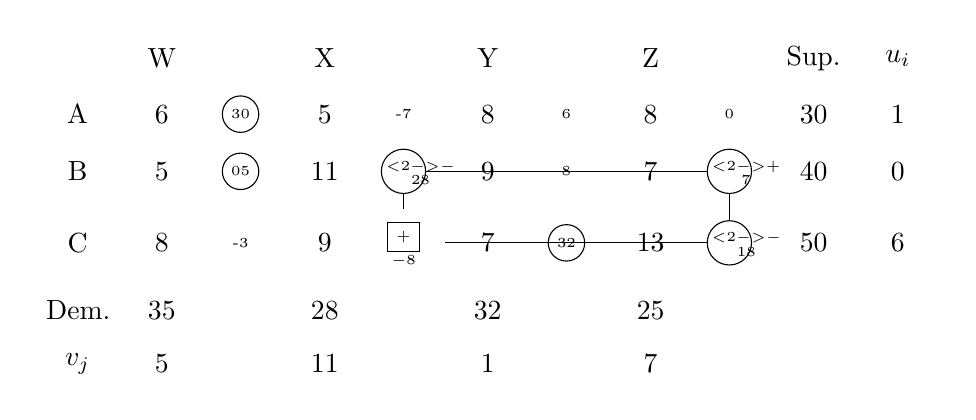
\begin{tikzpicture}
    \matrix(dd)[nodes={draw=none},align=center,text width=.8cm,
        row sep=0.2cm,column sep=1pt] {
                 & \node[]{W};                                     & \node[]{X};                                                                      & \node[]{Y};                                      & \node[]{Z};                                                        & \node[]{Sup.}; & \node[]{$u_i$}; \\
 \node[]{A};     & \node(d11)[]{6}; \circled{a1}{d11}{30}          & \node(d12)[]{5}; \node[right of=d12]{\tiny -7};                                  & \node(d13)[]{8}; \node[right of= d13]{\tiny 6};  & \node(d14)[]{8}; \node[right of=d14]{\tiny 0};                     & \node[]{30};   & {\node[]{1};}   \\
 \node[]{B};     & \node(d21)[]{5}; \circled{a2}{d21}{05}          & \node(d22)[]{11}; \circled{a3}{d22}{{$\stackrel{\only<2->{-}}{28}$}}             & \node(d23)[]{9};  \node[right of= d23]{\tiny 8}; & \node(d24)[]{7}; \circled{a4}{d24}{{$\stackrel{\only<2->{+}}{7}$}} & \node[]{40};   & {\node[]{0};}   \\
 \node[]{C};     & \node(d31)[]{8}; \node[right of=d31]{\tiny -3}; & \node(d32)[]{9}; \node(a8)[right of=d32]{\tiny $\stackrel{\fbox{+}}{\tiny -8}$}; & \node(d33)[]{7}; \circled{a5}{d33}{32}           & \node(d34)[]{13}; \circled{a6}{d34}{$\stackrel{\only<2->{-}}{18}$} & \node[]{50};   & {\node[]{6};}   \\
 \node[]{Dem.};  & \node[]{35};                                    & \node[]{28};                                                                     & \node[]{32};                                     & \node[]{25};                                                       &                &                 \\
 \node[]{$v_j$}; & {\node[]{5};}                                   & {\node[]{11};}                                                                   & {\node[]{1};}                                    & {\node[]{7};}                                                      &                &                 \\
    };
   \visible<2->{\draw[-](a8)--(a3);}
   \visible<2->{\draw[-](a3)--(a4);}
   \visible<2->{\draw[-](a4)--(a6);}
   \visible<2->{\draw[-](a6)--(a8);}
\end{tikzpicture}
\end{frame}

\begin{frame}[fragile]
\frametitle{Iteration 1}
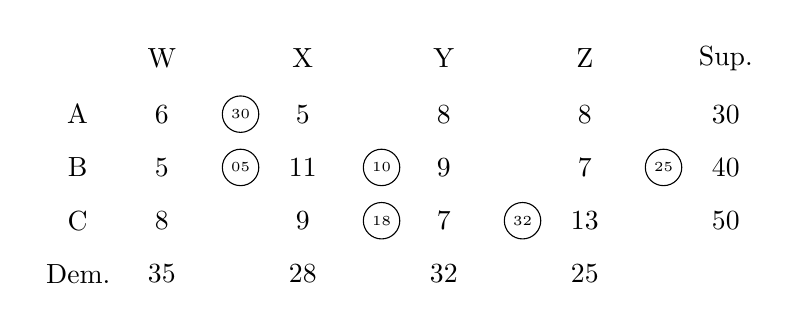
\begin{tikzpicture}
    \matrix(dd)[nodes={draw=none},align=center,text width=.8cm,
        row sep=0.2cm,column sep=1pt] {
                & \node[]{W};                            & \node[]{X};                             & \node[]{Y};                            & \node[]{Z};                       & \node[]{Sup.}; \\
 \node[]{A};    & \node(d11)[]{6}; \circled{a1}{d11}{30} & \node[]{5};                             & \node[]{8};                            & \node[]{8};                       & \node[]{30};   \\
 \node[]{B};    & \node(d21)[]{5}; \circled{a2}{d21}{05} & \node(d22)[]{11}; \circled{a3}{d22}{10} & \node(d23)[]{9};                       & \node[]{7}; \circled{a4}{d23}{25} & \node[]{40};   \\
 \node[]{C};    & \node[]{8};                            & \node(d32)[]{9};  \circled{a8}{d32}{18} & \node(d33)[]{7}; \circled{a5}{d33}{32} & \node(d34)[]{13};                 & \node[]{50};   \\
 \node[]{Dem.}; & \node[]{35};                           & \node[]{28};                            & \node[]{32};                           & \node[]{25};                      &                \\
    };
\end{tikzpicture}
\end{frame}

\begin{frame}[fragile]
\frametitle{Iteration 2}
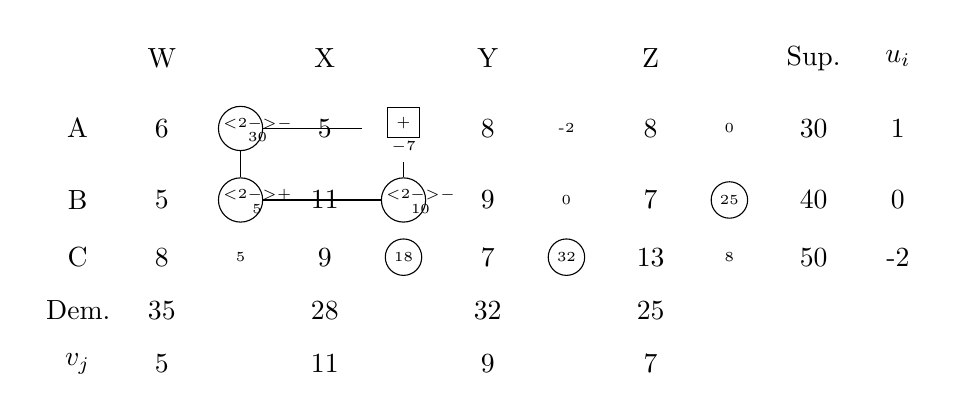
\begin{tikzpicture}
    \matrix(dd)[nodes={draw=none},align=center,text width=.8cm,
        row sep=0.2cm,column sep=1pt] {
                 & \node[]{W};                                                         & \node[]{X};                                                                & \node[]{Y};                                      & \node[]{Z};                                      & \node[]{Sup.}; & \node[]{$u_i$}; \\
 \node[]{A};     & \node(d11)[]{6}; \circled{a1}{d11}{{$\stackrel{\only<2->{-}}{30}$}} & \node(d12)[]{5}; \node(a7)[right of=d12]{\tiny $\stackrel{\fbox{+}}{-7}$}; & \node(d13)[]{8}; \node[right of= d13]{\tiny -2}; & \node(d14)[]{8}; \node[right of=d14]{\tiny 0};   & \node[]{30};   & {\node[]{1};}   \\
 \node[]{B};     & \node(d21)[]{5}; \circled{a2}{d21}{{$\stackrel{\only<2->{+}}{5}$}}  & \node(d22)[]{11}; \circled{a3}{d22}{{$\stackrel{\only<2->{-}}{10}$}}       & \node(d23)[]{9};  \node[right of= d23]{\tiny 0}; & \node(d24)[]{7}; \circled{a4}{d24}{{25}}         & \node[]{40};   & {\node[]{0};}   \\
 \node[]{C};     & \node(d31)[]{8}; \node[right of=d31]{\tiny 5};                      & \node(d32)[]{9}; \circled{a5}{d32}{18}                                     & \node(d33)[]{7}; \circled{a6}{d33}{32}           & \node(d34)[]{13}; \node[right of= d34]{\tiny 8}; & \node[]{50};   & {\node[]{-2};}  \\
 \node[]{Dem.};  & \node[]{35};                                                        & \node[]{28};                                                               & \node[]{32};                                     & \node[]{25};                                     &                &                 \\
 \node[]{$v_j$}; & {\node[]{5};}                                                       & {\node[]{11};}                                                             & {\node[]{9};}                                    & {\node[]{7};}                                    &                &                 \\
    };
   \visible<2->{\draw[-](a1)--(a2);}
   \visible<2->{\draw[-](a3)--(a2);}
   \visible<2->{\draw[-](a7)--(a3);}
   \visible<2->{\draw[-](a7)--(a1);}
\end{tikzpicture}
\end{frame}

\begin{frame}[fragile]
\frametitle{Iteration 2}
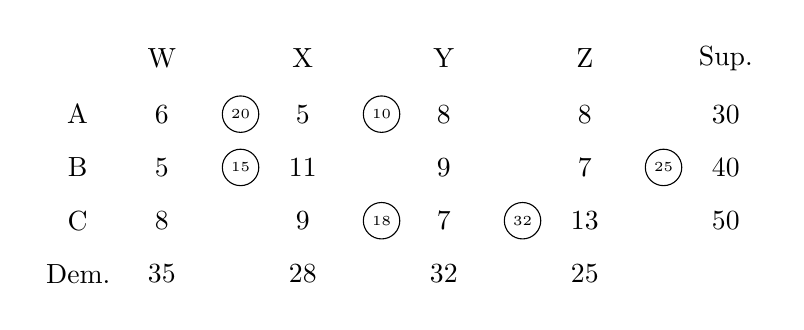
\begin{tikzpicture}
    \matrix(dd)[nodes={draw=none},align=center,text width=.8cm,
        row sep=0.2cm,column sep=1pt] {
                & \node[]{W};                            & \node[]{X};                             & \node[]{Y};                            & \node[]{Z};                       & \node[]{Sup.}; \\
 \node[]{A};    & \node(d11)[]{6}; \circled{a1}{d11}{20} & \node(d12)[]{5};  \circled{a2}{d12}{10} & \node[]{8};                            & \node[]{8};                       & \node[]{30};   \\
 \node[]{B};    & \node(d21)[]{5}; \circled{a3}{d21}{15} & \node(d22)[]{11};                       & \node(d23)[]{9};                       & \node[]{7}; \circled{a4}{d23}{25} & \node[]{40};   \\
 \node[]{C};    & \node[]{8};                            & \node(d32)[]{9};  \circled{a8}{d32}{18} & \node(d33)[]{7}; \circled{a5}{d33}{32} & \node(d34)[]{13};                 & \node[]{50};   \\
 \node[]{Dem.}; & \node[]{35};                           & \node[]{28};                            & \node[]{32};                           & \node[]{25};                      &                \\
    };
\end{tikzpicture}
\end{frame}

\begin{frame}[fragile]
\frametitle{Iteration 3}
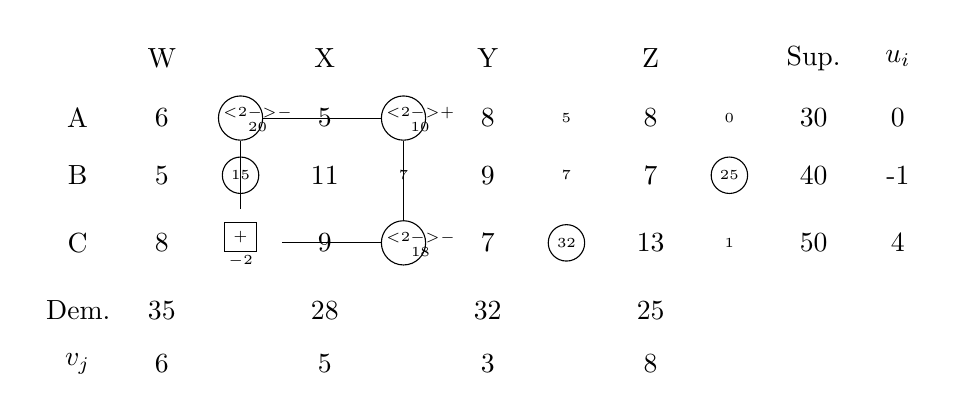
\begin{tikzpicture}
    \matrix(dd)[nodes={draw=none},align=center,text width=.8cm,
        row sep=0.2cm,column sep=1pt] {
                 & \node[]{W};                                                                & \node[]{X};                                                       & \node[]{Y};                                      & \node[]{Z};                                      & \node[]{Sup.}; & \node[]{$u_i$}; \\
 \node[]{A};     & \node(d11)[]{6}; \circled{a1}{d11}{{$\stackrel{\only<2->{-}}{20}$}}        & \node(d12)[]{5}; \circled{a2}{d12}{$\stackrel{\only<2->{+}}{10}$} & \node(d13)[]{8}; \node[right of= d13]{\tiny 5};  & \node(d14)[]{8}; \node[right of=d14]{\tiny 0};   & \node[]{30};   & {\node[]{0};}   \\
 \node[]{B};     & \node(d21)[]{5}; \circled{a3}{d21}{15}                                     & \node(d22)[]{11};  \node[right of=d22]{\tiny 7};                  & \node(d23)[]{9};  \node[right of= d23]{\tiny 7}; & \node(d24)[]{7}; \circled{a4}{d24}{{25}}         & \node[]{40};   & {\node[]{-1};}  \\
 \node[]{C};     & \node(d31)[]{8}; \node(a7)[right of=d31]{\tiny $\stackrel{\fbox{+}}{-2}$}; & \node(d32)[]{9}; \circled{a5}{d32}{$\stackrel{\only<2->{-}}{18}$} & \node(d33)[]{7}; \circled{a6}{d33}{32}           & \node(d34)[]{13}; \node[right of= d34]{\tiny 1}; & \node[]{50};   & {\node[]{4};}   \\
 \node[]{Dem.};  & \node[]{35};                                                               & \node[]{28};                                                      & \node[]{32};                                     & \node[]{25};                                     &                &                 \\
 \node[]{$v_j$}; & {\node[]{6};}                                                              & {\node[]{5};}                                                     & {\node[]{3};}                                    & {\node[]{8};}                                    &                &                 \\
    };
   \visible<2->{\draw[-](a1)--(a2);}
   \visible<2->{\draw[-](a2)--(a5);}
   \visible<2->{\draw[-](a7)--(a5);}
   \visible<2->{\draw[-](a7)--(a1);}
\end{tikzpicture}
\end{frame}

\begin{frame}[fragile]
\frametitle{Iteration 3}
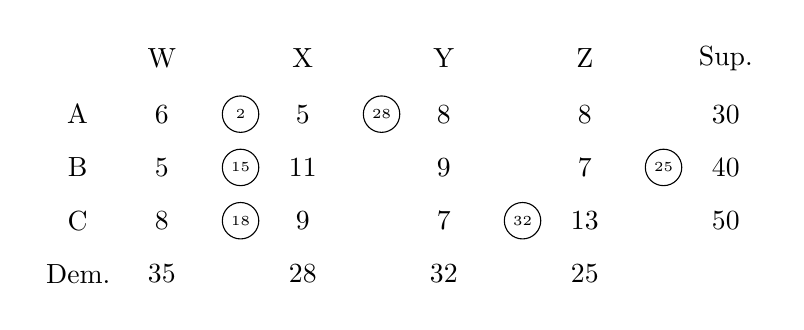
\begin{tikzpicture}
    \matrix(dd)[nodes={draw=none},align=center,text width=.8cm,
        row sep=0.2cm,column sep=1pt] {
                & \node[]{W};                            & \node[]{X};                             & \node[]{Y};                            & \node[]{Z};                            & \node[]{Sup.}; \\
 \node[]{A};    & \node(d11)[]{6}; \circled{a1}{d11}{2}  & \node(d12)[]{5};  \circled{a2}{d12}{28} & \node[]{8};                            & \node[]{8};                            & \node[]{30};   \\
 \node[]{B};    & \node(d21)[]{5}; \circled{a3}{d21}{15} & \node(d22)[]{11};                       & \node(d23)[]{9};                       & \node(d24)[]{7}; \circled{a4}{d24}{25} & \node[]{40};   \\
 \node[]{C};    & \node[]{8};    \circled{a5}{d11}{18}   & \node(d32)[]{9};                        & \node(d33)[]{7}; \circled{a5}{d33}{32} & \node(d34)[]{13};                      & \node[]{50};   \\
 \node[]{Dem.}; & \node[]{35};                           & \node[]{28};                            & \node[]{32};                           & \node[]{25};                           &                \\
    };
\end{tikzpicture}
\end{frame}

\begin{frame}[fragile]
\frametitle{Iteration 4}
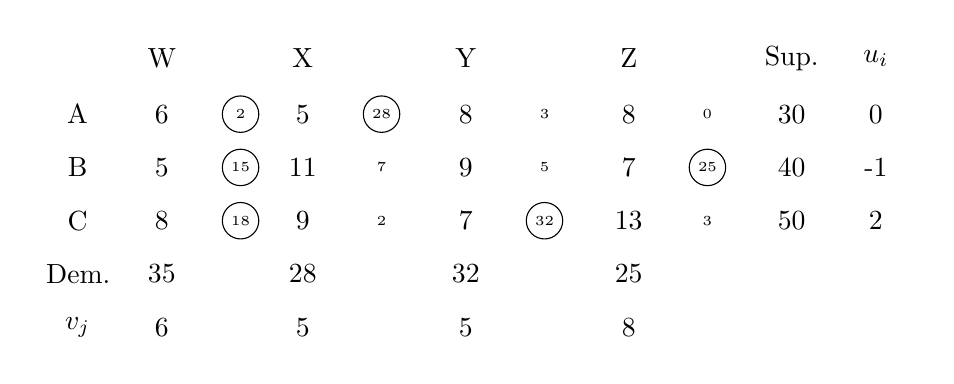
\begin{tikzpicture}
    \matrix(dd)[nodes={draw=none},align=center,text width=.8cm,
        row sep=0.2cm,column sep=1pt] {
                 & \node[]{W};                            & \node[]{X};                                      & \node[]{Y};                                      & \node[]{Z};                                      & \node[]{Sup.}; & \node[]{$u_i$}; \\
 \node[]{A};     & \node(d11)[]{6}; \circled{a1}{d11}{2}  & \node(d12)[]{5}; \circled{a2}{d12}{28}           & \node(d13)[]{8}; \node[right of= d13]{\tiny 3};  & \node(d14)[]{8}; \node[right of=d14]{\tiny 0};   & \node[]{30};   & {\node[]{0};}   \\
 \node[]{B};     & \node(d21)[]{5}; \circled{a3}{d21}{15} & \node(d22)[]{11};  \node[right of=d22]{\tiny 7}; & \node(d23)[]{9};  \node[right of= d23]{\tiny 5}; & \node(d24)[]{7}; \circled{a4}{d24}{{25}}         & \node[]{40};   & {\node[]{-1};}  \\
 \node[]{C};     & \node(d31)[]{8}; \circled{a5}{d21}{18} & \node(d32)[]{9}; \node[right of=d32]{\tiny 2};   & \node(d33)[]{7}; \circled{a6}{d33}{32}           & \node(d34)[]{13}; \node[right of= d34]{\tiny 3}; & \node[]{50};   & {\node[]{2};}   \\
 \node[]{Dem.};  & \node[]{35};                           & \node[]{28};                                     & \node[]{32};                                     & \node[]{25};                                     &                &                 \\
 \node[]{$v_j$}; & {\node[]{6};}                          & {\node[]{5};}                                    & {\node[]{5};}                                    & {\node[]{8};}                                    &                &                 \\
    };
\end{tikzpicture}
All the difference values are non-negative, hence the current BFS is optimal.
\end{frame}

\end{document}
